\chapter{文章}

\section{NFSS}
%*** LaTeX2e for class and package writers [#o7b142ef]
There is nothing to say for me.

\section{ベタ書きコマンドの簡易版\texorpdfstring{\zdash}{---}\Y{cmtt}}
%*** The ''cmtt'' package by Mark Wooding [#l45349b4]
\C{verb} コマンドはマクロの引数のなかで使えないとかで、状況に
よってはちょっと不便です。 \C{texttt} コマンドはタイプライタ体を出力するため
の命令ですが、特殊文字の \verb|$|, \verb|#|, \verb|\| などをタイプライタ
体で出力したいときには \verb|\{| や \verb|\_| とするとローマン体になり、
しょんぼりしてしまいます。そこで、 \ppl{Mark Wooding}の \Y{cmtt} を使う
事を考えます。これは
\begin{Syntax}
\C{mttfamily}
\C{textmtt}\pa{テキスト}
\end{Syntax}
の二つの宣言型と命令型のコマンドを使用できるようになります。
\C{textmtt} と同様に \C{mtt} も使えますので、次のように \C{mtt} を使うと
特殊記号等もタイプライタ体で出力できることでしょう。
\begin{InOut}
\usepackage{cmtt}
\mtt{\\, \{, \}, \_, \^, \$, \%}
\mtt{\&, \#, \~, \", \' \ , \|, \`}
\end{InOut}


\section{番号付箇条書き環境の拡張\texorpdfstring{\zdash}{---}\Y{enumerate}}

番号付の箇条書き環境 \E{enumerate} の拡張を \ppl{David Carlisle}が行な
い、これを \Y{enumerate} パッケージとして用いることができます。
\C{Alph}, \C{alph}, \C{Roman}, \C{roman}, \C{arabic} という命令の変わり
に、次の文字 (トークン) によってカウンタとすべき\Z{修飾子}を決めます。
\begin{Syntax}
A $=$ \C{Alph} \\
a $=$ \C{alph} \\
I $=$ \C{Roman} \\
i $=$ \C{roman} \\
1 $=$ \C{arabic}
\end{Syntax}
修飾子としたい文字は絶対に 波括弧 \{ \} でグルーピングしません。逆に
修飾子と区別が付かない文字列 (Exmaple, A などなど) はグルーピングします。
まずは、使用例を吟味してください。
\begin{InOut}
\usepackage{okumacro,graphicx}
\usepackage{enumerate}
\begin{enumerate}[{例題} 1]
  \item\label{exe:a} ほげほげ。
   \begin{enumerate}[{問題 \ref{exe:a}}-1]
    \item これはどうかな。
    \item それはどうです。
   \end{enumerate}
  \item ありゃま。
  \item こりゃま。
\end{enumerate}
\end{InOut}
\Z{丸数字}で番号付けをしたいとき等は \Y{okumacro} パッケージの \C{MARU} 命令
を使います。このような特殊なケースは \Y{enumerate} パッケージを使わずに直
接 \C{labelenumi} などのラベル部分を再定義した方がすんなりできる場合もあ
ります。
\begin{inputex}
\begin{enumerate}
%\renewcommand\labelenumi{\MARU{\arabic{enumi}}}
\item \TeX
\item \LaTeX\,2.09
\item \LaTeXe
\item \LaTeX\,3
\end{enumerate} 
\end{inputex}

%*** The epsfig package by Sebastian Rahtz [#gc099c0a]
%昔の ''psfig'' を模倣する互換性保持のためのパッケージなので、これも説明
%は省略。


\section{文字一覧の表示\texorpdfstring{\zdash}{---}\fl{fontsmpl.tex}}
%*** A font sampler by Alan Jeffrey [#wb3d74c3]
あるファミリーのフォント一覧 (シリーズやシェイプを含む) を表示させるには
\ppl{Alan Jeffrey}による \Fl{fontsmpl.tex} を用いると良いでしょう。
\type{latex fontsmpl}
とすると
\begin{OutTerm}
\family=
\end{OutTerm}
と聞かれるので、適当に \type{cmr} などとすると、\fl{fontsmpl.dvi} 
が作成されるので、その出力ファイルの内容を吟味してください。


%\section{footnote}
% \Y{footnote} パッケージを使わずに、別のアプローチで
% \E{table}/\E{tabular} 環境中の \C{footnote} を出力する方法を紹介してい
% るので省略。

\section{版面の設定\texorpdfstring{\zdash}{---}\Y{geometry}}

なんだかんだいって \LaTeXe で版面を構築するのは面倒なもんです。
\ppl{梅木秀雄}による \Y{geometry} パッケージを使うことで、結構簡単に
設定しなおすことができます。
\begin{inputex}
\usepackage[margin=2cm]{geometry}
\end{inputex}
とかすると、上下左右の余白が ちょうど 2\,cm になります。
\begin{inputex}
\usepackage[papersize={width,height}]{geometry}
\end{inputex}
の \va{width}, \va{height} に用紙の\va{幅}/\va{高さ}を設定したり
\begin{inputex}
\usepackage[paper=a4paper]{geometry}
\end{inputex}
とか、色々できます。詳しくは付属のマニュアルをご覧ください。

\section{見出し直後の字下げ\texorpdfstring{\zdash}{---}\Y{indentfirst}}
%*** The indentfirst package by David Carlisle [#d5fb7795]
欧文の場合、章見出しや節見出しの直後の段落は字下げしない (字下げしなくとも
段落が始まることが明白) という慣習があるので、\C{chapter} と
か \C{section} のあとは \C{if@afterindent} なる命令が偽 (\C{iffalse}) に
なることにより、字下げしないようになります。時として日本語を欧文のクラス
ファイルで組むときにこれがお節介をするので
\begin{inputex}
\usepackage{indentfirst}
\end{inputex}
とすると見出し直後の段落も字下げするようになります  (本当に欧文の
文書を作成するときは、\Y{indentfirst} パッケージを読み込まない
方が自然です)。

%\section{Displaying page \Y{layout} valiables}
%\Y{layout} パッケージは初級編で説明しているので省略。

%\section{\Y{leftidx} package} 
%初級編および論文作成の手引で既出。


\section{多段組み\texorpdfstring{\zdash}{---}\Y{multicol}}

\LaTeXe の標準では \C{onecolumn} と \C{twocolumn} によって 1 段組みと 2 段組みを
切替えることも出来ますし、
\begin{inputex}
\documentclass[twocolumn]{jsarticle}
\end{inputex}
によって全体の段組みを指定することも出来ます。しかし、 \C{onecolumn} と \C{twocolumn}
の両方とも改ページが必須で、ページの途中で段を変更することも出来なければ、
2 段組みのときに段の終わりが揃わないなどの制約あります (普通の組版規則では
ページの途中で段を変更するようなことはないので、これはこれで良いのだが)。
これを解消するためには \ppl{Frank Mittelbach}の作成した (\emph{\TeX
book} の多段組みアルゴリズムをベースに) \Y{multicol} パッケージを用いる
と良いでしょう。%ただし、商用使用には payment とか donate とか色々。
\begin{Syntax}
\C{begin}\verb|{multicols*}|\pa{段数}\opa{多段組みを行なう前のテキスト}\\
\va{多段組みを行なう要素}\\
\C{end}\verb|{multicols*}|
\end{Syntax}
星を付けると段の下端を揃えないようにするので、通常は星無しで用いると良いでしょう。
%例えば、次のようなファイルがあるとします。
\Y{multicol} パッケージの制約として \E{table} 環境や \E{figure} 環境
で図表を出力することができません。そのかわり \E{table*} 環境並びに
E{figure*} 環境で段を打ち抜いて図表を出力することが出来ます。
この場合はページの上端か下端に配置されるようになります。
余白等を手動で調整する手間を惜しまないならば、次の入力例のように
自前の \E{mytable} 環境や \E{myfigure} 環境を定義することが出来ます。
%
\begin{inputex}
\documentclass[a4j,10pt,papersize]{jsarticle}
\newcommand*\mypict{\setlength\unitlength{1pt}%
  \begin{picture}(40,40)%
    \put(20,20){\circle*{10}}%
    \put(20,20){\circle{20}}%
  \end{picture}}%
\usepackage{multicol}
\columnseprule=.4pt
\columnsep=2zw
\multicolsep=1zw
\makeatletter
\def\myfigure{\vbox\bgroup\centering\def\@captype{figure}}
\def\mytable{\vbox\bgroup\centering\def\@captype{table}}
\def\endmyfigure{\egroup}
\def\endmytable{\egroup}
\def\hoge{\@tempcnta=\z@ \@whilenum \@tempcnta<100\do{%
   ほげほげ\advance\@tempcnta\@ne}。}
\makeatother
\begin{document}
\hoge
\begin{multicols}{3}
\hoge
\begin{equation}
 f(x)  = ax +b
\end{equation}
\hoge
\begin{figure*}[tb]
\centering\mypict
\caption{普通の\texttt{figure}環境での図だよ}
\end{figure*}
\hoge
\begin{myfigure}
 \mypict
 \caption{\texttt{multicols}環境中の図だよ}
\end{myfigure}
\hoge
\begin{mytable}
\begin{small}
  \caption{\texttt{multicols}環境中の表だよ}
 \begin{tabular}{lll}
 \hline
 \LaTeX & \LaTeXe& \LaTeX\,3\\
 \hline
 \end{tabular}
\end{small}
\end{mytable}
\hoge
\end{multicols}
\hoge
\begin{multicols}{4}[\section{新聞記事とか色々あるけどねぇ、どうだろう。}]
\hoge
\end{multicols}
\hoge
\begin{multicols}{5}
\hoge\par \hoge
\end{multicols}
\hoge 
\begin{multicols}{7}
\hoge\par \hoge
\end{multicols}
\end{document}
\end{inputex}
上記の入力例の出力例は\figref{fig:multicol}となります。
\begin{figure}[htbp]
   \IOmargin
   \makebox[0pt][l]{%
      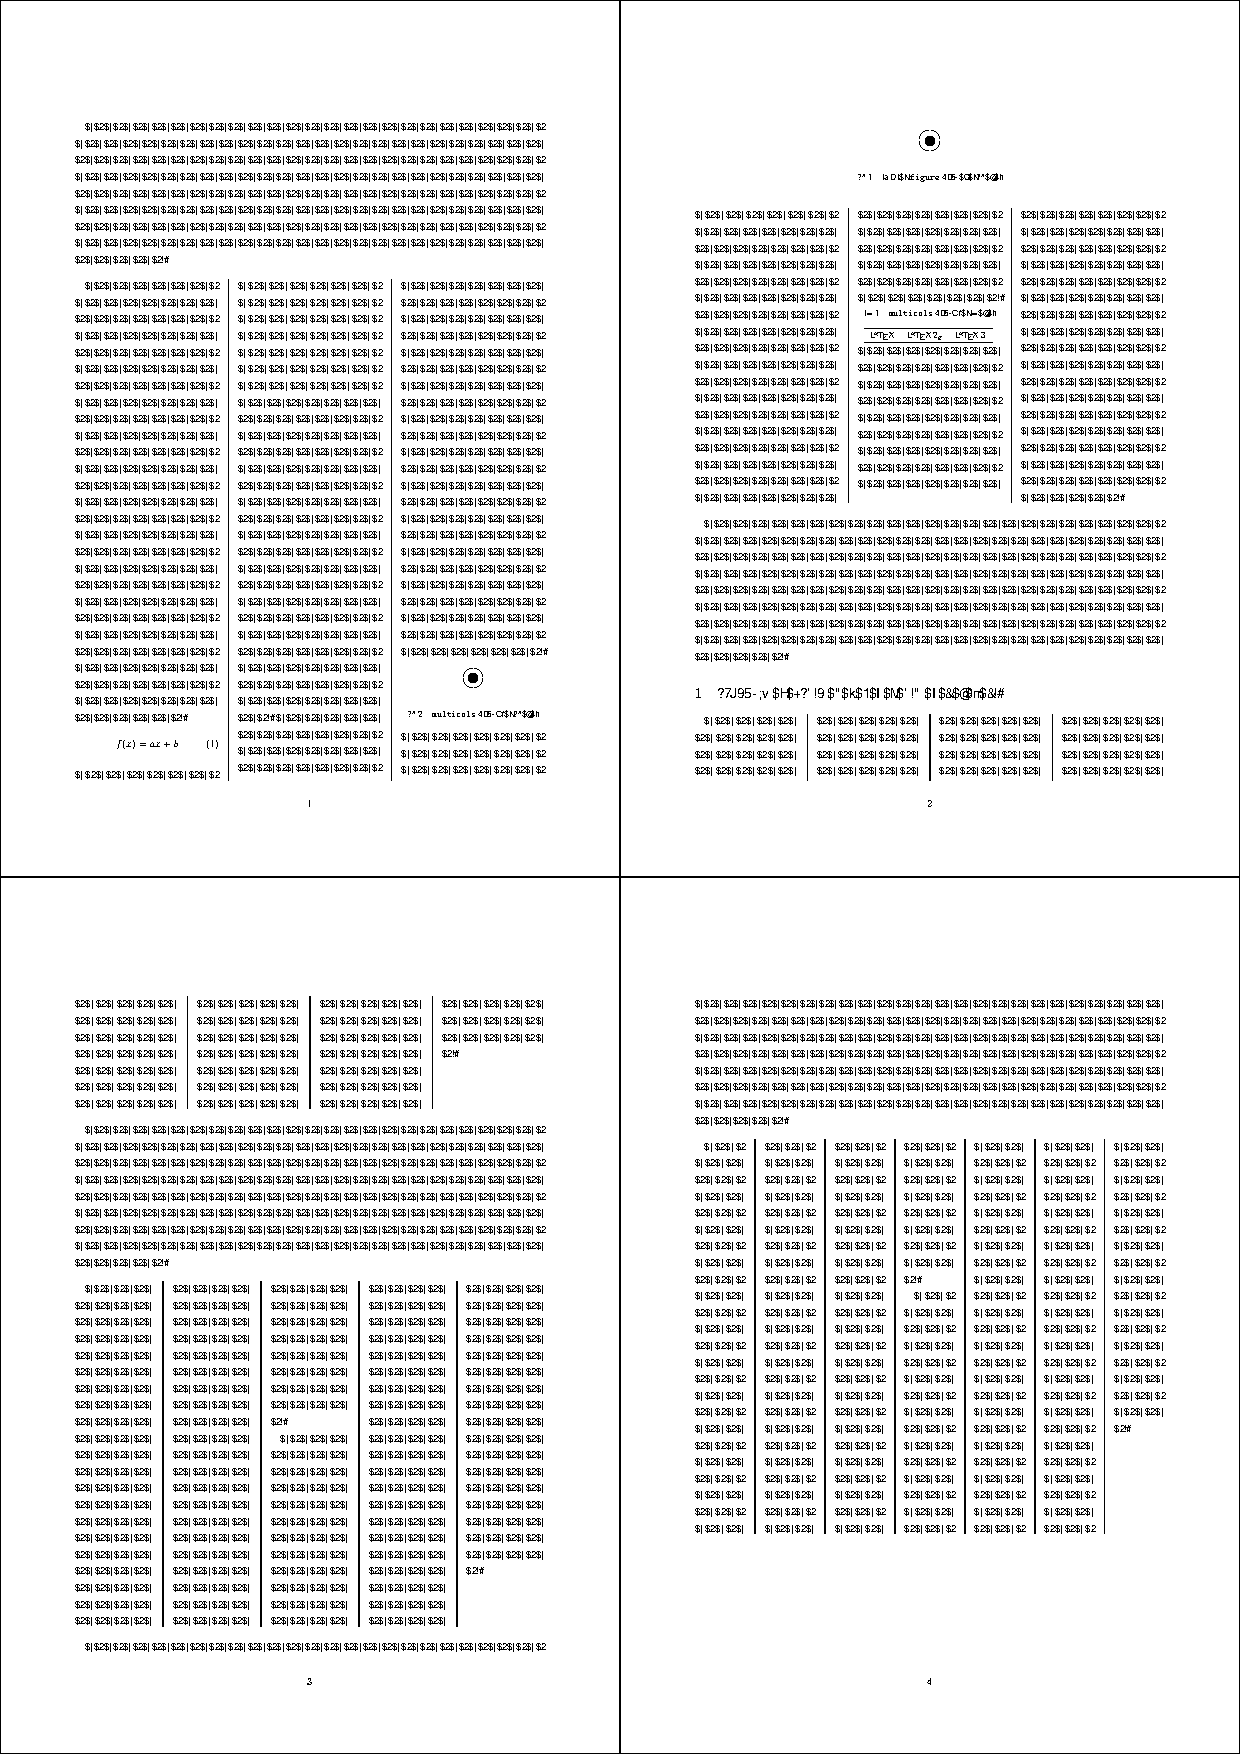
\includegraphics[width=\fullwidth]{images/multicol}%
   \IOlabel
   }%
   \caption{\Y{multicol}の使用例の出力結果}\label{fig:multicol}%
\end{figure}
\ppl{Frank Mittelbach}の \Y{multicol} では 段抜きで配置する \E{figure*}
環境と \E{table*} 環境は許されますが、段の中に組まれる \E{figure}/\E{table}
環境は使えません。そのため、図をフロートさせずに配置するために
\E{myfigure}/\E{mytable} 環境を新設しています。ただし、フロートしないの
で図表の直前/直後で余計な空白が挿入されるので、これを手動で調整する (具体的には
関係する文の少し後に \E{myfigure}/\E{mytable} を記述する) ことになります。

段間の空白、段間に引かれる罫線、段の上端/下端の空きは次のように設定しま
す。 
\begin{inputex}
\columnseprule=.4pt % 段間に引かれる罫線
\columnsep=2zw %  段間の空白
\multicolsep=1zw % 段の上端/下端の空き
\end{inputex}

%*** url [#l5e85cd4]
%手引と初級編で紹介済み。

%*** cite [#qe8a7ba0]
%手引と初級編で紹介済み。
\section{2段組での脚注の体裁調整\texorpdfstring{\zdash}{---}\Y{ftnright}}
2 段組以上において、\LaTeXe の標準の脚注出力では、左右の段のいずれかに
出力されますが、これを右側にだけ (3 段組み以上の場合はページの最後の段だ
け) に出力する \ppl{Frank Mittelbach}による \Y{ftnright} があります。
\begin{inputex}
\documentclass[twocolumn]{jsarticle}
% \footnoterule の定義を保存
\let\origfootnoterule\footnoterule
\usepackage{ftnright}
\global\let\footnoterule\origfootnoterule
\usepackage{ifthen}
\newcounter{hoge}
\newcommand\hoge[1][1000]{\whiledo{\value{hoge}<#1}{%
  \stepcounter{hoge}ほげ}\footnote{脚注なり。}。\setcounter{hoge}{0}}
\gdef\footnoterule{\kern-3pt \hrule width .4\columnwidth \kern 2.6pt}
\begin{document}
\author{An Author}
\title{A Title}
\maketitle
\section{はじめの節}
\hoge[50] \hoge[50] \hoge[70] \hoge[100]
\section{次の節}
\hoge \hoge[20] \hoge[30] \hoge[50]
\end{document}
\end{inputex}
基本的には 2 段組み以上で \Y{ftnright} パッケージを読み込むだけで良いのですが、
\C{footnoterule} が引かれないので、これを
\begin{inputex}
\let\origfootnoterule=\footnoterule
\usepacckage{ftnright}
\global\let\footnoterule=\origfootnoterule
\end{inputex}
として定義しなおした方が良いでしょう、上記のファイルの出力例は
\figref{fig:ftnright}となります。

\begin{figure}[htbp]
   \IOmargin
   \makebox[0pt][l]{%
      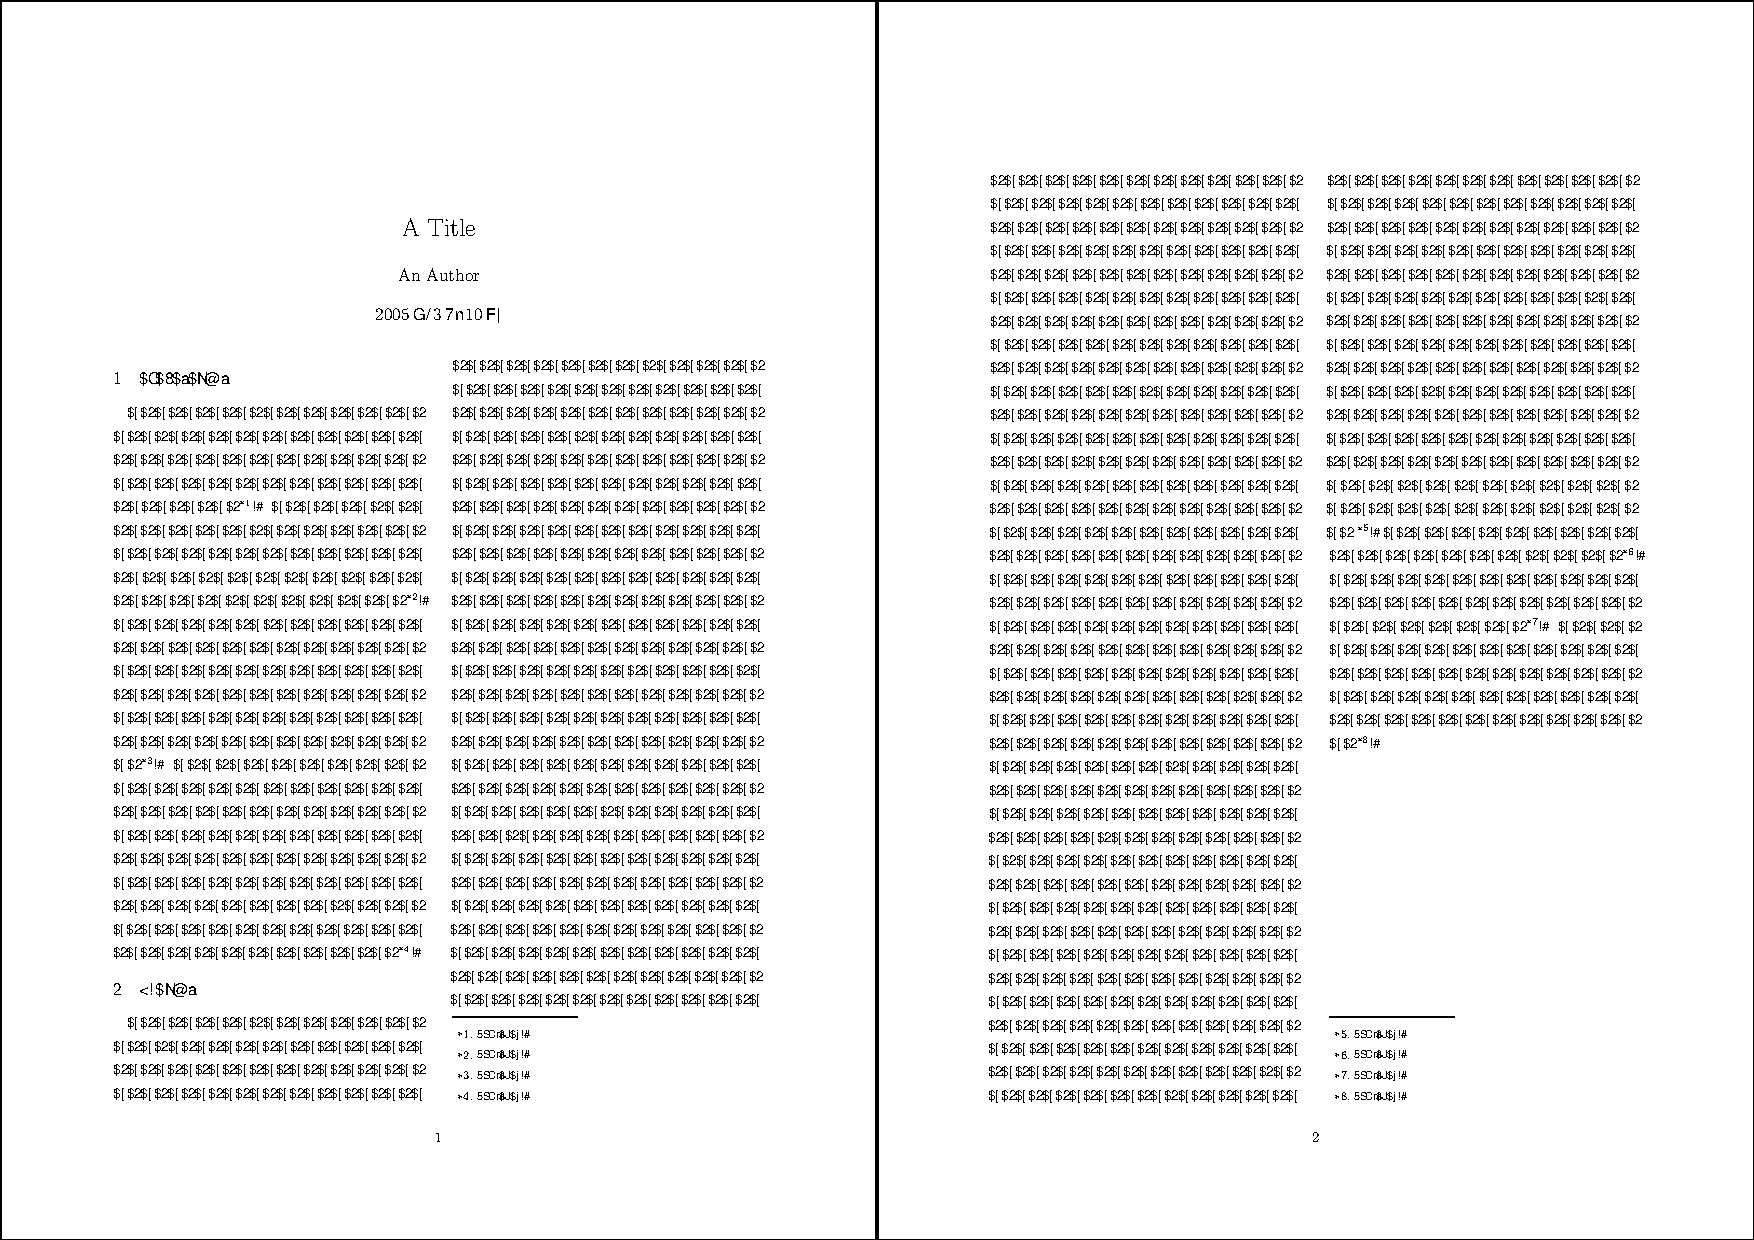
\includegraphics[height=\fullwidth,angle=-90]{images/ftnright}%
   \IOlabel
   }%
   \caption{\Y{ftnright}の使用例の出力結果}\label{fig:ftnright}%
\end{figure}


%*** endnotes (後注 [#l65c94f7]
\section{\Z{後注}\texorpdfstring{\zdash}{---}\Y{endnotes}}
とある学会のスタイルで注釈は巻末にまとめること、などという歴史的な
指定をされることがあります\footnote{実際、脚注を活版印刷で入れるのは結構
技術が必要とされるし、途中で原稿が変更されると組み直し等を余儀なくされ、
注釈はすべて後注として先に組んでおいた方が楽であったという歴史背景があり
ます。}。\Y{endnotes} パッケージでは \C{footnote} 命令や \C{marginpar}
命令を書き換えるわけではなく、新規に \C{endnotes} という命令を提供
しています。
\begin{Syntax}
\va{用語}\C{endnotes}\pa{用語の注釈}
\end{Syntax}
\Y{endnotes}パッケージは次のように使用すると良いでしょう。
\begin{inputex}
\documentclass{jsbook}
\usepackage{endnotes}
\def\notesname{注釈}
\begin{document}
ほげほげ\endnote{ほげほげとはほげほげなのでほげである。}
%
\newpage% ここから注釈のページのはじまり
\begingroup
\parindent = 0pt
\def\enotesize{\normalsize}
\theendnotes
\endgroup 
\end{document}
\end{inputex}


%//** footbib (脚注に参考文献
%//参考文献を巻末ではなく、それぞれ参照しているページの脚注に
%//表示させたい場合があります。これには Eric Domenjoud による footbib 
%//が使えるかも知れません。

% hoge hoge hoge
\section{ハンギング\texorpdfstring{\zdash}{---}\Y{dropping}}
% hoge hoge hoge
欧文の雑誌や書籍では \Z{initial-cap} と呼ばれるもの、段落始めの頭文字を
おおきく見せる装飾が良く見受けられます。これを実現するには、自分で
マクロを書いても良いのですが (中級編で解説します)、既存の \Y{dropping} を
使う方法があります。\Y{graphicx} パッケージに依存しますが、欧文の場合は
満足の行く出力結果となることでしょう。
\begin{Syntax}
\C{dropping}\pa{頭文字のために確保する行数}\pa{頭文字} \va{通常の段落要素}
\end{Syntax}

\Y{dropping}パッケージのより \C{dropping} 命令が使えるようになり、
\begin{InOut}
\usepackage{dropping}
%\section{dropping}
\dropping{3}{\sffamily{} This} is a very 
 simple sample file fordropping package. 
`Hoge' is hoge hoge.
\end{InOut}
% hoge hoge hoge
`This' の部分がサンセリフ体で 3 行分の大きさで {dropping} 
されます。宣言型の書体変更コマンドを用いる場合はその宣言のすぐあとに
波括弧 \verb|{}| を挿入しなければなりません。


\section{Texinfo もどき\texorpdfstring{\zdash}{---}\Y{at}}

\Prog{Texinfo} の\Z{エスケープ文字}はアットマーク `@' です。
\LaTeX も \Z{バックスラッシュ} `\textbackslash'です。Texinfo もどきにエ
スケープ文字をアットマークに変更することもできます。これには
\ppl{Mark Wooding}による \Y{at} パッケージが使えることでしょう。

さほど使う人もいないと思われるので、入力例だけを示して終わりにしましょう。
\begin{inputex}
\documentclass{jsarticle}
\usepackage{at,makeidx}
\newatcommand sec[1]{\section{#1}}
\newatcommand ssec[1]{\subsection{#1}}
\newatcommand sssec[1]{\subsubsection{#1}}
\makeindex
\newatcommand showindex{\printindex}
\atdef|#1|{\texttt{#1}}
\begin{document}
@sec{ほげ}
@/hogehoge/ @@
@ssec{ほげほげ}
@*hogehoge*
@sssec{ほげほげほげ}
@|TypeWriter|, Hoge@i{hoge} is @I{hoge}.
@showindex
\end{document}
\end{inputex}


